\chapter{Conclusion and Future Work}
\section{Conclusion}
This thesis focuses on human detection in enclosed industrial environments with UWB radar. This research is performed in collaboration with industry, it faces a real world application where the requirements are well defined and rigid, where a false alarm can be costly in robotic or a mining applications and a missed target can mean injuries and loss of lives. 

A successful target detection is a combination of two parts, first the chosen system hardware/technology should able to detect the target in the environment it is intended to be used in. The second part is dealing with the filtering and processing of the acquired signals and how efficient these methods are therefore the focus of this thesis was to investigate what the system is capable of, it's constraints and processing of the obtained signals. This has so far resulted in three peer-reviewed publications. 
%The areas that have been looked into are radar signal processing in time domain, statistical signal processing and detection theory. 

There are several challenges for reaching the research goal (see \ref{ProblemFormulation}). Based of the  measurements in the office environment and published in paper B the probability of false alarm is around 50 percent. This is not a satisfactory result and needs further investigation. In addition discrimination of a human from other object is not an easy task. Spatio-temporal properties of a dynamic human body such as arm and hand movements could be a discerned by micro-Doppler processing but in case of static humans the chest movement during breathing could not deliver satisfactory results in a real world scenario and needs further investigations. Furthermore based on the Mie theory presented in paper C the 1-3 GHz system does not provide the best discerning for human body and use of lower frequencies is recommended.

\section{Future Work}
Future work can be directed in different paths which some of them are presented in this chapter.

During this research some of the system characteristics such as precision and effect of environment noise in signal detection were measured and defined whereas some other characteristics such as maximum range needs to be measured and defined. Furthermore some investigation is needed to figure out how much of the high percentage of the false alarm depends on the signal processing algorithms and how much is system/hardware dependent.

Using Multipe Input Multiple Output (MIMO) system can reveal more details about the targets and therefore could reveal more details about the target. 

On other possibility is to use sensor fusion to take advantage of each sensor strength to increased confidence of detection and decrease false alarms. combination of radar sensor with cameras seems like a


\subsection{Machine Learning and AI(Deep Learning)}
This study,focuses on studying the detection of a human
target’s status behind wall. The auto-encoder(AE) algorithm is applied. In the context of small sample conditions, the states of behind-wall human targets
are classified and identified with a single sensor and multiple sensors. Furthermore, the results are compared with
other classification algorithms. Improving the classification and identification rates(ref?)more results?

\todo{Gait analysis?}
Human gait has been analyzed extensively in Vision and Ultrasound applications \cite{Littel2003497}, \cite{LeeGaitAnalyze}, \cite{wan2018survey}, \cite{NixonAutomaticgait}. To estimate human walking parameters a model is needed. There are some models developed for different applications such as Thalmann model \cite{Thalman}.The model describes the dynamics of the human body parts as a function of time. In \cite{VanDorp} Thalmann model is used to estimate human walking parameters. Radar equipment is also modeled, radar equation is used to calculate each human body part and calculates the spectrogram from it. The fit function calculates the difference between the simulated and measured radar data and adjust the parameters of the walking model.\todo{This work could just show that it is possible to animate a human walking by building a model based on radar measurements. Shall I write it here or not?}
\begin{figure}
  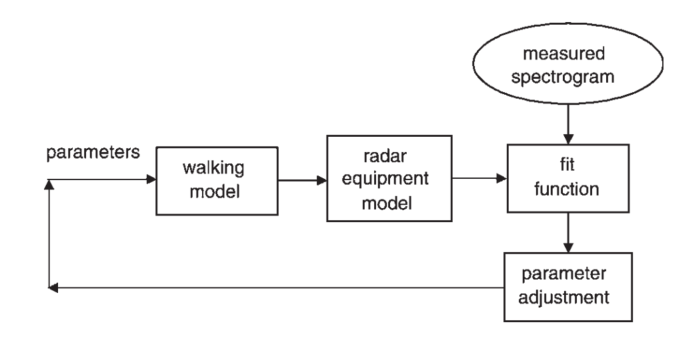
\includegraphics[width=0.9\textwidth]{Figures/ModelBasedApproach.PNG}
  \caption{Model Based Approach\cite{VanDorp}}
  \label{fig:ModelBasedApproach}
\end{figure}

\begin{figure}
  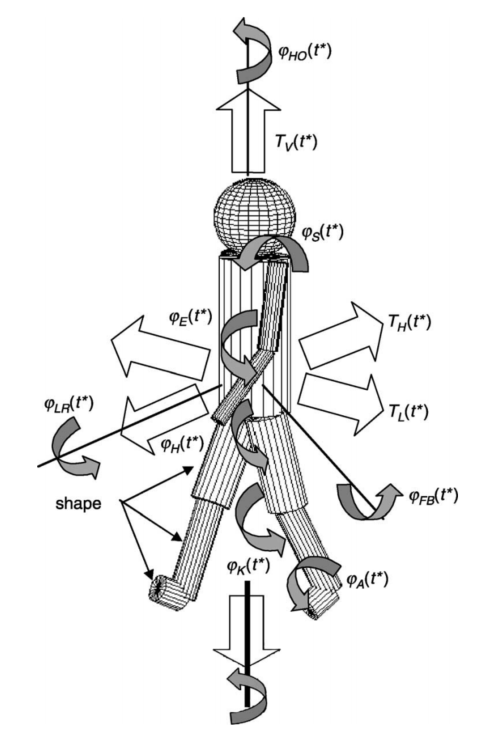
\includegraphics[width=0.5\textwidth]{Figures/HumanModel.PNG}
  \caption{Human model with 12 body parts, 3 translation
trajectories and 14 rotation trajectories\cite{VanDorp}}
  \label{fig:HumanModel}
\end{figure}